\documentclass[preprint,12pt,authoryear=false]{elsarticle}
% Target journal: Computers & Security (Elsevier). Elsevier's elsarticle class, numeric citations.
\usepackage{amsmath,amssymb}
\usepackage{graphicx}
\usepackage{booktabs}
\usepackage{multirow}
\usepackage{xcolor}
\usepackage[hidelinks]{hyperref}
\usepackage{lineno}
\usepackage{siunitx}
\usepackage{pifont}
\usepackage{adjustbox}
\makeatletter\newcommand{\tabinput}[1]{\@@input #1 }\makeatother
\journal{Computers \& Security}
\biboptions{numbers,sort&compress}

\begin{document}
\begin{frontmatter}

\title{Beyond benchmark accuracy: a joint evaluation of cross-dataset shift, unseen attack families and calibration for budget-constrained intrusion-detection triage}

% TODO(author): add affiliations and e-mail addresses before submission.
\author[aff1]{Osman Can Çetlenbik\corref{cor1}}
\ead{[e-mail]}
\author[aff2]{Ahmet Ali Süzen}
\cortext[cor1]{Corresponding author.}
\affiliation[aff1]{organization={[Department, University]},
            city={[City]},
            country={Türkiye}}
\affiliation[aff2]{organization={[Department, University]},
            city={[City]},
            country={Türkiye}}

\begin{abstract}
Machine-learning intrusion detectors report near-perfect accuracy on public benchmarks, yet their behaviour in deployment is poorly understood. Deployment brings three challenges at once: traffic from a different network, attack families absent from training, and an analyst team that can review only a fixed number of alerts. A recent review found that no study published between 2024 and 2026 evaluated these concerns together. We present a joint evaluation of four model families on five public benchmarks (CIC-IDS2017, CSE-CIC-IDS2018, ACI-IoT-2023, UNSW-NB15 and ToN-IoT), covering six directed cross-dataset pairs over a harmonised 77-feature flow representation and 47 leave-one-family-out experiments, with discrimination, calibration, base-rate precision and review-budget metrics reported side by side. We also propose a budgeted conformal triage that tests each flow against the hypothesis ``benign and typical of training traffic'' by fusing detector and novelty p-values calibrated on benign flows. In-domain, all models reach AUROC 0.96--0.99, with calibration error at most 0.002 after isotonic recalibration. Across datasets, AUROC falls to 0.50--0.62 and calibration error rises to 0.24--0.45, and recalibration on source data does not repair it. Transferred thresholds either raise the false-positive rate 5--32-fold or detect only 2--3\% of attacks. Within a dataset, 14 of 47 unseen families are detected less than half of the time, 11 of them with over half of their flows given an attack probability below 0.05. Enforcing the review budget with a quantile of unlabeled target traffic keeps the median queue size within 5\% of plan under every shift, whereas transferred thresholds miss it by factors of 0.4 to 54. Fisher fusion of novelty and detector evidence roughly doubles recall at a 1\% budget on the families the detector misses (0.07 to 0.15) at a cost of up to 6 points on families it already detects. Code, data provenance and all results are released.
\end{abstract}


\begin{keyword}
Network intrusion detection \sep Machine learning \sep Distribution shift \sep Calibration \sep Conformal prediction \sep Zero-day attacks \sep Alert triage
\end{keyword}

\end{frontmatter}

\section{Introduction}\label{sec:intro}

Machine-learning-based network intrusion detection systems (NIDS) routinely report accuracies and F1 scores above 0.99 on public benchmarks, yet practitioners remain reluctant to deploy them~\cite{sommer2010outside,arp2022dos,apruzzese2023sok}. A large part of the gap is that benchmark numbers answer a question operators do not ask. A security operations centre (SOC) does not need a classifier that separates benign and attack flows in a random split of one capture. It needs a system that, on \emph{its own} network, with \emph{today's} attacks and with a \emph{fixed} number of analyst hours, puts the right flows in front of analysts and does not bury them in false alarms~\cite{alahmadi2022falsepositives}. Three properties matter for that goal. The detector must transfer to traffic that differs from its training data (cross-dataset or domain shift)~\cite{layeghy2023explainable,cantone2024cross}. It must not silently wave through attack families it has never seen (open-set or zero-day behaviour)~\cite{talpini2024enhancing,farrukh2023detecting}. And its confidence must mean something, so that thresholds and alert volumes can be planned (calibration)~\cite{guo2017calibration,pal2025calibrated}. Because attacks are rare, all three must be judged at realistic base rates, where even a small false-positive rate dominates the alert queue~\cite{axelsson2000base}.

Each of these properties has been studied, but almost always in isolation. Cross-dataset studies show that performance can drop sharply when a model trained on one benchmark is applied to another~\cite{layeghy2023explainable,cantone2024cross,xin2025crossdataset}; open-set studies hold out attack classes within one dataset~\cite{talpini2024enhancing,farrukh2023detecting,yu2025industrial}; calibration and uncertainty studies typically stay in-distribution or within a single dataset~\cite{pal2025calibrated}; and conformal methods for security have focused on malware concept drift~\cite{jordaney2017transcend,barbero2022transcending} or adversarial perturbations~\cite{li2026robust,yumlembam2024comprehensive}. A recent review of 29 empirical deep-learning NIDS studies published between 2024 and 2026 found that \emph{none} evaluated cross-dataset generalisation, rejection of unseen attack families and confidence reliability together~\cite{lew2026deployment}. The closest empirical work evaluates calibration and fixed-false-positive-rate alerting under cross-dataset transfer, but for binary detection only, without unseen families or selective and conformal mechanisms, and with a single seed~\cite{jin2026benchmark}.

This paper closes that gap with a joint, budget-aware evaluation and a simple triage mechanism that can be added to any detector. Our contributions are:
\begin{enumerate}
\item \textbf{A joint evaluation protocol.} We evaluate four standard model families on five public benchmarks under three regimes (in-domain, six directed cross-dataset pairs over a harmonised 77-feature CICFlowMeter space, and leave-one-family-out), with five seeds. We report discrimination, calibration, false-alarm inflation, base-rate precision and analyst-budget metrics side by side, so that the same model can be judged on all of them at once.
\item \textbf{Budgeted conformal triage.} We frame alert triage as testing the null hypothesis ``benign and typical of the training traffic'' and combine a detector-based and a novelty-based conformal p-value calibrated on benign flows only. The resulting queue has a distribution-free false-alarm guarantee under exchangeability, and its size can be fixed to the SOC budget from \emph{unlabeled} target traffic.
\item \textbf{Empirical findings.} We quantify how far in-domain calibration and false-alarm guarantees survive under each type of shift, how often unseen attack families are missed with high confidence, and when novelty evidence helps or hurts a budgeted review queue (Section~\ref{sec:results}).
\item \textbf{Reproducibility.} All code, dataset provenance (URLs, commit hashes and checksums) and raw result tables are released, and every number in this paper is produced by that code.
\end{enumerate}

The remainder of the paper is organised as follows. Section~\ref{sec:related} reviews related work. Section~\ref{sec:method} describes the data, protocols and triage method. Section~\ref{sec:results} presents the results, Section~\ref{sec:discussion} discusses implications and threats to validity, and Section~\ref{sec:conclusion} concludes.

\section{Related work}\label{sec:related}

\paragraph{Evaluation pitfalls in ML-based NIDS} Sommer and Paxson~\cite{sommer2010outside} argued early that anomaly detection in networks differs fundamentally from typical ML settings: errors are expensive, the base rate of attacks is low~\cite{axelsson2000base}, and there is a semantic gap between alerts and actionable incidents. Arp et al.~\cite{arp2022dos} systematised pitfalls such as sampling bias, data snooping and inappropriate baselines, and Apruzzese et al.~\cite{apruzzese2023sok} called for assessments that reflect operational constraints. Several works document quality problems in the benchmarks themselves: labelling and feature-extraction errors in CIC-IDS2017~\cite{engelen2021troubleshooting,lanvin2023errors}, and ``design smells'' such as poor diversity and ill-defined generalisation criteria across seven datasets~\cite{flood2024bad}. Standardised NetFlow feature sets were proposed to enable comparison across datasets~\cite{sarhan2021netflow,sarhan2022standard,sarhan2022evaluating}, and temporal re-analyses of those datasets have recently been released~\cite{luay2025temporal}. In malware detection, TESSERACT~\cite{pendlebury2019tesseract} showed how spatial and temporal bias inflates results, and Apruzzese et al.~\cite{apruzzese2024adversarial} examined how drift interacts with adversarial perturbation in NIDS.

\paragraph{Cross-dataset generalisation} Layeghy and Portmann~\cite{layeghy2023explainable} and Cantone et al.~\cite{cantone2024cross} report near-perfect in-dataset performance that drops to near chance across datasets. Xin and Xu~\cite{xin2025crossdataset} add Platt-scaled calibration and AUC-oriented training to a transformer and evaluate across NSL-KDD, UNSW-NB15 and CIC-IDS2017. Jin and Lee~\cite{jin2026benchmark} harmonise features across HIKARI-2021, CIC-IDS2017 and CICIoT2023 and show that a 5\% false-positive-rate threshold chosen in-domain does not hold after transfer, even when ranking metrics look good. These studies treat detection as binary and do not examine unseen attack families or selective or conformal alerting.

\paragraph{Unseen attacks and uncertainty} Open-set NIDS approaches reject unknown attacks with clustering~\cite{farrukh2023detecting} or prototype learning with extreme-value thresholds~\cite{yu2025industrial}. Talpini et al.~\cite{talpini2024enhancing} compare uncertainty-quantification methods, including Bayesian neural networks, for detecting held-out attack classes, and Pal et al.~\cite{pal2025calibrated} study calibration and uncertainty for IoT attack detection under within-dataset shift. General-purpose baselines for misclassification and out-of-distribution detection include maximum softmax probability~\cite{hendrycks2017baseline} and energy scores~\cite{liu2020energy}; Ovadia et al.~\cite{ovadia2019trust} showed that calibration degrades under dataset shift, with ensembles~\cite{lakshminarayanan2017simple} among the most robust options. Post-hoc calibration methods include Platt scaling~\cite{platt1999probabilistic}, isotonic regression~\cite{zadrozny2002transforming,niculescu2005predicting} and Bayesian binning~\cite{naeini2015obtaining}.

\paragraph{Conformal and selective prediction in security} Conformal prediction provides distribution-free guarantees under exchangeability~\cite{vovk2022algorithmic,lei2018distribution,angelopoulos2023conformal}, with extensions to covariate shift~\cite{tibshirani2019conformal}, online adaptation~\cite{gibbs2021adaptive}, non-exchangeable data~\cite{barber2023conformal}, risk control~\cite{angelopoulos2024conformal} and outlier testing with conformal p-values~\cite{bates2023testing}. Selective classification trades coverage for accuracy~\cite{geifman2017selective}. In security, Transcend~\cite{jordaney2017transcend,barbero2022transcending} and CADE~\cite{yang2021cade} use conformal evaluators or contrastive embeddings to detect drifting malware samples. For intrusion detection, Yumlembam et al.~\cite{yumlembam2024comprehensive} add a conformal rejection layer to an adversarially hardened botnet detector, and Li~\cite{li2026robust} restores conformal coverage under adversarial feature perturbation for LLM-based detectors. Neither considers natural cross-dataset shift, unseen families or an analyst budget.

\paragraph{Positioning} Table~\ref{tab:positioning} summarises the dimensions covered by the closest works. To our knowledge, this is the first study to evaluate cross-dataset shift, unseen attack families, calibration and conformal or selective alerting \emph{jointly} and under an explicit analyst budget, as called for by a recent review~\cite{lew2026deployment}.

\begin{table}[t]
\centering
\caption{Coverage of deployment concerns in closely related work (\checkmark: evaluated; $\circ$: partially). XD: cross-dataset shift; OS: unseen attack families; CAL: probability calibration; AB: alert budget or fixed false-positive-rate operation; CP/SEL: conformal or selective prediction.}\label{tab:positioning}
\small
\begin{adjustbox}{max width=\linewidth}
\begin{tabular}{lccccc}
\toprule
Work & XD & OS & CAL & AB & CP/SEL\\
\midrule
Talpini et al.~\cite{talpini2024enhancing} & & \checkmark & \checkmark & & \\
Pal et al.~\cite{pal2025calibrated} & $\circ$ & $\circ$ & \checkmark & & \\
Xin and Xu~\cite{xin2025crossdataset} & \checkmark & & \checkmark & & \\
Cantone et al.~\cite{cantone2024cross} & \checkmark & & & & \\
Yumlembam et al.~\cite{yumlembam2024comprehensive} & & & & & \checkmark\\
Li~\cite{li2026robust} & $\circ$ & & & & \checkmark\\
Jin and Lee~\cite{jin2026benchmark} & \checkmark & & \checkmark & \checkmark & \\
\textbf{This work} & \checkmark & \checkmark & \checkmark & \checkmark & \checkmark\\
\bottomrule
\end{tabular}
\end{adjustbox}
\end{table}

\section{Evaluation framework and triage method}\label{sec:method}

\subsection{Problem setting}
A flow-based NIDS observes a stream of flow records $x\in\mathbb{R}^d$ and must decide which flows to surface to a security operations centre (SOC). Each flow has a binary label $y\in\{0,1\}$ (benign/attack) and, for attacks, a family label $f$. A detector $h$ trained on a \emph{source} dataset outputs a score $s(x)=\hat{P}(y=1\mid x)$. At deployment the detector meets a \emph{target} stream whose distribution can differ from the source in two ways that we study separately: (i)~\emph{cross-dataset shift}, where the network, capture tooling and attack implementations change (benign and attack distributions both move); and (ii)~\emph{unseen-family shift}, where the network is the same but an attack family absent from training appears. We call the setting with neither shift \emph{in-domain}.

We take the SOC's point of view and assume that analysts can inspect at most a fraction $b$ of the flows in a stream (the \emph{review budget}), and that attacks are rare. Unless stated otherwise the target streams have attack prevalence $\pi=1\%$ and budgets are $b\in\{1\%,2\%,5\%\}$; a perfect ranker therefore reaches full recall for every $b\ge\pi$.

\subsection{Datasets and harmonisation}\label{sec:data}
We use five public benchmarks (Table~\ref{tab:data}). Three of them, CIC-IDS2017~\cite{sharafaldin2018toward}, CSE-CIC-IDS2018 (the AWS-hosted ``Processed Traffic Data for ML Algorithms'' release) and ACI-IoT-2023, were produced with CICFlowMeter and share 76 flow features plus the transport protocol; we align them column by column (the 2018 naming is canonical) and verify the alignment programmatically with a token-level name check. These three datasets support cross-dataset experiments in both directions. UNSW-NB15~\cite{moustafa2015unsw} (official training and testing partitions, merged) and the network part of ToN-IoT have their own feature sets and are used for in-domain and unseen-family experiments. We remove identifiers that act as shortcuts or do not transfer (flow IDs, IP addresses, ports, timestamps), one-hot encode low-cardinality categorical fields (UNSW-NB15 and ToN-IoT, top-15 values per field), replace non-finite values by zero, and remove exact duplicates over features and label. To keep the study computationally balanced, we then cap benign flows at 200{,}000 and each attack family at 30{,}000 per dataset by uniform sampling; for CSE-CIC-IDS2018, benign flows are first Bernoulli-subsampled at 5\% while streaming the 16.2~million rows. Families are also mapped to coarse groups (DoS, DDoS, Scan, BruteForce, WebAttack, Botnet, Infiltration) for the cross-dataset analysis. The exact provenance (URLs, commit hashes, checksums) is listed in the supplementary repository.

The CIC-IDS2017 copy we could obtain is the stratified subsample released by the mlp4nids project (all attack flows, roughly a quarter of the benign flows), and the ToN-IoT copy retains 50{,}000 of the 300{,}000 normal records of the official train--test file. Because we resample to fixed prevalences for every operational metric, these subsampling choices affect the benign diversity available for training, not the metrics' definitions; we return to this in Section~\ref{sec:threats}.

\subsection{Detectors and calibration}
We evaluate four widely used model families: LightGBM~\cite{ke2017lightgbm} (300 trees, 63 leaves), random forest~\cite{breiman2001random} (150 trees), a multilayer perceptron (128--64 units, early stopping) and logistic regression, all from scikit-learn~\cite{pedregosa2011scikit} or the LightGBM library. Inputs are transformed with a signed $\log(1+|x|)$ followed by standardisation fitted on the training split. Each source dataset is split, stratified by family, into training (50\%), calibration (20\%) and test (30\%) partitions; all results are repeated over five seeds that change both the split and the model initialisation.
Probabilities are post-processed with Platt scaling~\cite{platt1999probabilistic} or isotonic regression~\cite{zadrozny2002transforming} fitted on the source calibration split, and we report expected calibration error (ECE, 15 equal-width bins)~\cite{naeini2015obtaining,guo2017calibration} and the Brier score.

\subsection{Operating points and base rates}
Following common practice, the alert threshold $\tau_\alpha$ is set on the source calibration split so that the benign false-alarm rate is $\alpha=1\%$. On a target stream we measure the realised true-positive rate (TPR) and false-positive rate (FPR) at $\tau_\alpha$, the \emph{FPR inflation} $\mathrm{FPR}/\alpha$, and the precision the detector would achieve at attack prevalence $\pi$,
\begin{equation}
\mathrm{Prec}_\pi=\frac{\mathrm{TPR}\,\pi}{\mathrm{TPR}\,\pi+\mathrm{FPR}\,(1-\pi)},
\end{equation}
which makes the base-rate effect~\cite{axelsson2000base} explicit.

\subsection{Budgeted conformal triage}\label{sec:triage}
Ranking flows by $s(x)$ exploits what the detector has learned but cannot surface traffic that resembles nothing seen in training, which is precisely where unseen attacks and shifted traffic live~\cite{sommer2010outside}. We therefore formulate triage as testing, for each flow, the null hypothesis
\[
H_0(x):\ \text{``$x$ is benign and typical of the source traffic''},
\]
and review the flows with the strongest evidence against $H_0$. Two conformal p-values~\cite{vovk2022algorithmic,angelopoulos2023conformal,bates2023testing} are computed against the \emph{benign} flows of the source calibration split, $\mathcal{C}_0=\{x_i\}_{i=1}^{n}$:
\begin{align}
p_{\mathrm{det}}(x) &= \frac{1+\#\{i: s(x_i)\ge s(x)\}}{n+1}, &
p_{\mathrm{nov}}(x) &= \frac{1+\#\{i: u(x_i)\ge u(x)\}}{n+1},
\end{align}
where $u(x)$ is a novelty score, here the mean Euclidean distance to the $k=5$ nearest neighbours among up to 20{,}000 \emph{benign} training flows in the transformed feature space. $p_{\mathrm{det}}$ is small when the detector recognises attack-like behaviour; $p_{\mathrm{nov}}$ is small when the flow is atypical of the benign traffic the model was trained on, whether or not it resembles a known attack. Using benign flows as the reference matches the null hypothesis; in an ablation it also separated held-out families from benign traffic better than a reference that included training attacks (Section~\ref{sec:discussion}). We combine them either with a Bonferroni rule, $p_{\mathrm{B}}=\min\{1,2\min(p_{\mathrm{det}},p_{\mathrm{nov}})\}$, or with Fisher's method, $p_{\mathrm{F}}=1-F_{\chi^2_4}\!\big(-2\log p_{\mathrm{det}}-2\log p_{\mathrm{nov}}\big)$. If benign target flows are exchangeable with $\mathcal{C}_0$, each $p_{\mathrm{det}}$ and $p_{\mathrm{nov}}$ is super-uniform, and the Bonferroni rule $p_{\mathrm{B}}\le\alpha$ flags at most a fraction $\alpha$ of benign flows in expectation, whatever the dependence between the two scores. Fisher's rule is exact only under independence, so we use it purely as a ranking. Cross-dataset shift breaks exchangeability by design; one purpose of our experiments is to measure how much of the guarantee survives.

\paragraph{Budget enforcement without target labels} Given a budget $b$, the review queue consists of the flows whose priority $-\log p(x)$ exceeds a threshold $t_b$. We compare two ways of choosing $t_b$: (a)~\emph{source transfer}, the $(1-b)$-quantile of priorities on a source stream with the same prevalence; and (b)~\emph{label-free warm-up}, the $(1-b)$-quantile on the first 20\% of the unlabeled target stream, applied to the remaining 80\%. Option (b) needs no labels because a budget is a statement about volume, not about accuracy. We report the realised \emph{load} (queue size divided by $b\cdot N$; 1 means the budget is respected exactly) and the attack recall inside the queue. We also report the recall of the exact top-$b$ fraction of each stream, which isolates ranking quality from threshold selection.

\subsection{Experimental protocols}
\paragraph{Protocol XD (in-domain and cross-dataset)} For every source dataset, seed and model, we train on the source training split, calibrate on the source calibration split, and evaluate on the source test split (in-domain) and, for the three CICFlowMeter datasets, on the test split of each other dataset (six directed cross-dataset pairs). No target information is used except the unlabeled warm-up window of the budget rule.
\paragraph{Protocol OS (unseen families)} For every dataset and every attack family with at least 300 flows, we remove that family from the training and calibration splits and evaluate on the test split. The target stream contains all benign test flows plus the held-out family at 1\% prevalence, emulating a new campaign. We report the recall of the held-out family at $\tau_\alpha$, the fraction of its flows that the isotonic-calibrated detector labels benign with confidence above 95\% (\emph{confident misses}), and the triage metrics. This protocol uses LightGBM and three seeds.

\section{Results}\label{sec:results}

\begin{table}[t]
\centering
\caption{Datasets after harmonisation. ``Rows read'' counts the records loaded; for CSE-CIC-IDS2018 it is the count after the 5\% Bernoulli subsampling of benign rows during streaming (all attack rows kept). ``Dup.'' is the share of those rows removed as exact duplicates over features and label. Benign and attack counts are after the per-class caps.}\label{tab:data}
\small
\begin{adjustbox}{max width=\linewidth}
\begin{tabular}{lrrrrrr}
\toprule
Dataset & Rows read & Unique & Dup. (\%) & Benign & Attack & Families\\
\midrule
\tabinput{tables/data.tex}
\bottomrule
\end{tabular}
\end{adjustbox}
\end{table}

\subsection{Data quality}
Table~\ref{tab:data} summarises the data. Exact duplicates are pervasive: between 26\% (CIC-IDS2017) and 56\% (ToN-IoT) of the records we loaded are feature-and-label copies of another record. Duplication is concentrated in a few families; for example, only 1{,}956 of the roughly 159{,}000 PortScan flows in our CIC-IDS2017 copy are unique, and only 54 of the 193{,}360 FTP-BruteForce flows in CSE-CIC-IDS2018 are unique. A random split of the raw data therefore places identical flows in the training and test sets, which inflates in-domain scores. All results below are computed after deduplication.

\subsection{In-domain performance is near ceiling and well calibrated}
In-domain, every model separates benign from attack traffic almost perfectly on the three CICFlowMeter datasets (Table~\ref{tab:xd}; AUROC 0.964--0.993) and on UNSW-NB15 and ToN-IoT (AUROC 0.964--1.000; per-model values are in the released result tables). The tree ensembles and the MLP are already well calibrated (ECE $\le 0.008$), and isotonic regression brings every model to ECE $\le 0.002$. The false-positive rate at the threshold chosen on the calibration split matches its nominal value ($\mathrm{FPR}/\alpha = 1.0$). Even here, however, the base rate caps what an alert can mean. At 1\% attack prevalence, a detector with 96\% TPR and 1\% FPR yields a precision of only about 0.49, so every second alert is a false alarm.

\begin{table}[t]
\centering
\caption{In-domain versus cross-dataset performance on the three CICFlowMeter datasets (mean $\pm$ s.d.\ over five seeds; cross-dataset values are averaged over the six directed pairs first). $\mathrm{FPR}/\alpha$ is the realised false-positive rate at the source threshold divided by its nominal value $\alpha=1\%$. TPR is measured at the same threshold. $\mathrm{Prec}_{1\%}$ is the precision implied at 1\% attack prevalence.}\label{tab:xd}
\small
\setlength{\tabcolsep}{3.5pt}
\begin{adjustbox}{max width=\linewidth}
\begin{tabular}{llcccccc}
\toprule
Model & Setting & AUROC & ECE (raw) & ECE (iso) & $\mathrm{FPR}/\alpha$ & TPR & $\mathrm{Prec}_{1\%}$\\
\midrule
\tabinput{tables/xd_main.tex}
\bottomrule
\end{tabular}
\end{adjustbox}
\end{table}

\subsection{Cross-dataset shift breaks ranking, calibration and alert volume at once}
Across datasets, all four models collapse to near-chance ranking (mean AUROC 0.50--0.62; Table~\ref{tab:xd}). The best pair, CIC-IDS2017$\to$CSE-CIC-IDS2018, reaches only 0.78 with LightGBM, and ACI-IoT-2023$\to$CIC-IDS2017 is \emph{worse} than chance (0.45; Fig.~\ref{fig:heat}). Individual seed--model runs range from AUROC 0.25 to 0.81, so the outcome of a single transfer experiment is largely a matter of chance. Calibration fails with the ranking: ECE rises from $\le0.04$ to 0.24--0.45, and isotonic or Platt recalibration fitted on source data does not help (isotonic ECE 0.28--0.45), because the mapping it learns belongs to the source distribution.

The operating point fails in two opposite ways that the ranking metrics hide. Models trained on CIC-IDS2017 or CSE-CIC-IDS2018 \emph{flood} a new network with alarms: their realised FPR is 5 to 32 times the nominal 1\% (Fig.~\ref{fig:heat}, right). Models trained on ACI-IoT-2023 instead go \emph{silent}: they keep the FPR near its nominal value on the other networks (1.2$\times$) but detect only 2--3\% of the attacks. The implied precision at 1\% prevalence falls from 0.39--0.49 in-domain to 0.024--0.034 across datasets, meaning that about 97 of every 100 alerts would be false. Per-group recall shows that sharing an attack name does not guarantee transfer. The CSE-CIC-IDS2018 model detects 76\% of CIC-IDS2017 DoS flows but only 0.2\% of its DDoS flows, and the CIC-IDS2017 model detects 70\% of CSE-CIC-IDS2018 DoS flows but 0.6\% of its botnet flows (released per-group table).

\begin{figure}[t]
\centering
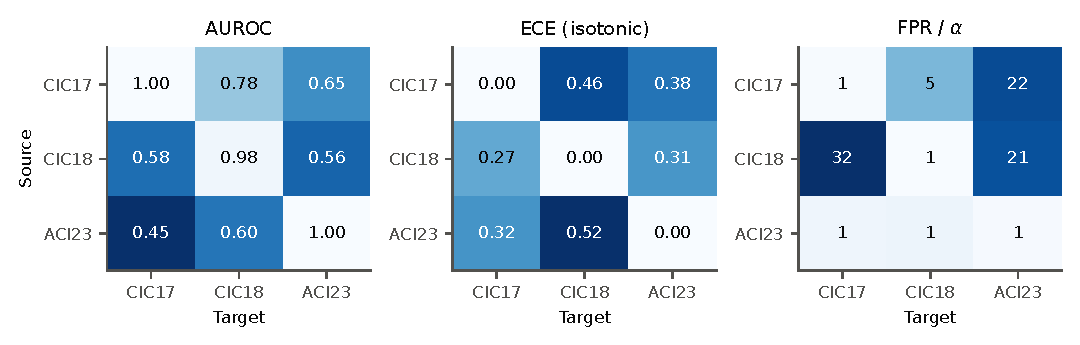
\includegraphics[width=\linewidth]{../figures/xd_heatmaps.pdf}
\caption{LightGBM trained on the row dataset and tested on the column dataset (mean over five seeds). Left: AUROC. Middle: ECE after isotonic calibration fitted on the source. Right: realised false-positive rate at the source threshold divided by the nominal 1\% (colour on a log scale). Diagonals are in-domain.}\label{fig:heat}
\end{figure}

\subsection{Unseen attack families are often missed, and missed confidently}
Holding out each of the 47 attack families with at least 300 flows, one at a time, lowers the median recall at the 1\% FPR threshold from 0.999 for the families seen in training to 0.847 for the held-out family (Table~\ref{tab:os}). The median hides a heavy tail: 14 of the 47 families (30\%) are detected less than half of the time. For 11 of them, more than half of the flows receive an isotonic-calibrated attack probability below 0.05, so the calibrated model is confidently wrong (Fig.~\ref{fig:os}). ACI-IoT-2023 is the extreme case: 7 of its 10 families fall below 50\% recall, and the median confident-miss rate is 0.96, because its floods and sweeps look nothing like the other attacks in the same dataset. CIC-IDS2017 Bot (recall 0.002) and SSH-Patator (0.09), CSE-CIC-IDS2018 Infiltration (0.03) and DDoS-LOIC-HTTP (0.03), and UNSW-NB15 Fuzzers (0.16) are other examples.

However, the information needed to find these flows is often present in the score. The AUROC between the held-out family and benign traffic stays high (median per dataset 0.90--0.996). The failure is therefore mainly one of \emph{thresholding}: the attack scores rise above benign scores, but not above a threshold tuned for the families the model already knows. This is what motivates reviewing flows by rank under a budget rather than by a fixed threshold.

\begin{table}[t]
\centering
\caption{Leave-one-family-out results with LightGBM (three seeds). Recall is measured at the source 1\%-FPR threshold. Median values are across held-out families. ``$<$0.5'' is the number of held-out families detected less than half of the time. ``Conf.\ miss'' is the median (maximum) fraction of held-out flows that the isotonic-calibrated model scores below 0.05. The two AUROC columns compare held-out flows with benign flows, using the detector score and the benign-referenced kNN novelty score respectively.}\label{tab:os}
\small
\setlength{\tabcolsep}{3.5pt}
\begin{adjustbox}{max width=\linewidth}
\begin{tabular}{lccccccc}
\toprule
Dataset & Fam. & Recall (seen) & Recall (unseen) & $<$0.5 & Conf.\ miss & AUROC det. & AUROC nov.\\
\midrule
\tabinput{tables/os_summary.tex}
\bottomrule
\end{tabular}
\end{adjustbox}
\end{table}

\begin{figure}[t]
\centering
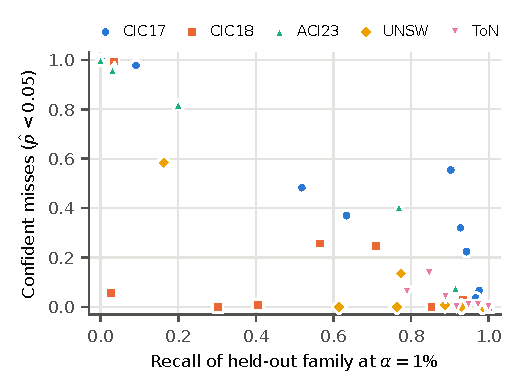
\includegraphics[width=0.62\linewidth]{../figures/os_scatter.pdf}
\caption{Each point is one held-out attack family (mean over three seeds). Points in the upper-left region are families the detector misses at its operating threshold \emph{and} labels benign with more than 95\% calibrated confidence.}\label{fig:os}
\end{figure}

\subsection{Budgeted triage}
Figure~\ref{fig:triage} and Table~\ref{tab:triage} report the fraction of attacks that land in the analyst queue when the queue holds the top 1\%, 2\% or 5\% of a stream with 1\% attack prevalence.

\paragraph{In-domain} Ranking by the detector score is best, capturing 89\%, 94\% and 96\% of attacks at the three budgets. Adding novelty evidence costs a little: Fisher fusion is lower by 2.5 points on average (Wilcoxon signed-rank $p<10^{-10}$ over 75 paired configurations), and novelty alone is poor (21--57\%), because known attacks need no novelty evidence.

\paragraph{Unseen families} Averaged over all 47 families, Fisher fusion and the detector score are statistically indistinguishable (mean difference $+1.0$ point, $p=0.29$ over 423 paired configurations). The average, however, mixes two groups with opposite behaviour (Table~\ref{tab:gain}). For the 14 families that the detector misses at its threshold, Fisher fusion doubles the recall inside a 1\% budget (0.072 to 0.152) and adds about 10 points at 2\% and 5\% ($p=4\times10^{-8}$; better in 68\% and worse in 20\% of paired configurations). For the 33 families the detector already catches, fusion costs up to 6 points at a 2\% budget. The Bonferroni rule is more conservative and brings no gain on either group. The grouping uses the held-out labels, so it explains where fusion helps but cannot serve as a deployment rule; Section~\ref{sec:discussion} discusses the trade-off.

\paragraph{Cross-dataset} No ranking rescues cross-dataset transfer. With a 5\% budget, every priority captures only 13--15\% of the attacks, against 5\% for a random queue of the same size.

\begin{figure}[t]
\centering
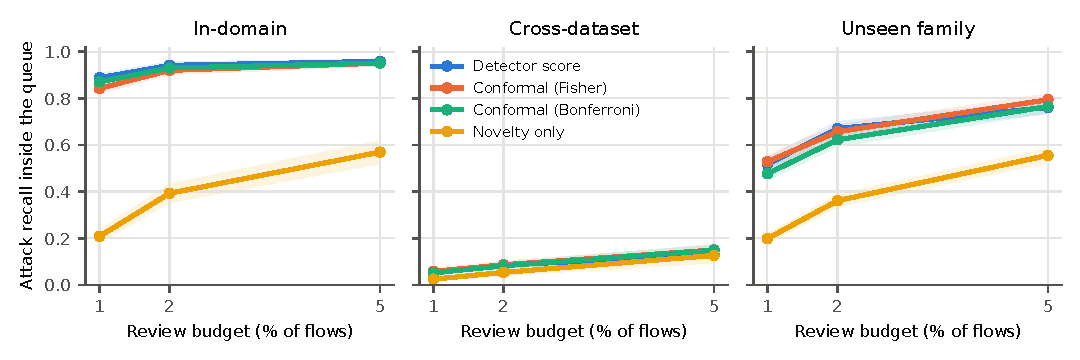
\includegraphics[width=\linewidth]{../figures/triage_recall.pdf}
\caption{Attack recall inside the review queue versus the review budget, for streams with 1\% attack prevalence (LightGBM; shaded bands are $\pm$1 standard error across configurations). The queue is the exact top-$b$ fraction of the stream by each priority.}\label{fig:triage}
\end{figure}

\begin{table}[t]
\centering
\caption{Attack recall inside the review queue (top-$b$ fraction of a stream with 1\% attack prevalence; LightGBM; mean over configurations).}\label{tab:triage}
\small
\begin{adjustbox}{max width=\linewidth}
\begin{tabular}{llccc}
\toprule
Regime & Priority & $b=1\%$ & $b=2\%$ & $b=5\%$\\
\midrule
\tabinput{tables/triage.tex}
\bottomrule
\end{tabular}
\end{adjustbox}
\end{table}

\begin{table}[t]
\centering
\caption{Unseen families: recall inside the queue, split by whether the detector's recall on the held-out family at the 1\%-FPR threshold is below 0.5. $\Delta$ is Fisher minus detector.}\label{tab:gain}
\small
\begin{adjustbox}{max width=\linewidth}
\begin{tabular}{lcccccc}
\toprule
Detector recall & Families & $b$ & Detector & Bonferroni & Fisher & $\Delta$\\
\midrule
\tabinput{tables/os_gain.tex}
\bottomrule
\end{tabular}
\end{adjustbox}
\end{table}

\subsection{Budgets can be enforced without target labels}
A review budget is only useful if the queue actually has the planned size. Table~\ref{tab:budget} and Fig.~\ref{fig:load} compare the two ways of setting the queue threshold for the Fisher priority. Transferring the threshold from the source works in-domain (median load 1.00--1.03). Under cross-dataset shift, the transferred threshold admits 20--54 times the planned volume at the median (the maximum possible load is $1/b$, i.e.\ the whole stream). The recall of 0.69--0.97 it reports in that setting is therefore an artefact of flagging almost everything. Under unseen-family shift, the transferred threshold instead leaves the queue at 38\% of its planned size at a 1\% budget and misses attacks the analysts had time to inspect. The label-free warm-up quantile keeps the median load between 0.98 and 1.05 in all three regimes (10th--90th percentile 0.84--1.34). With the queue size fixed, recall at a 1\% budget on unseen families rises from 0.41 to 0.53.

\begin{table}[t]
\centering
\caption{Budget adherence of the Fisher priority. ``Load'' is realised queue size divided by the planned size (median [10th, 90th percentile]); recall is attack recall inside the queue on the 80\% of the stream after the warm-up window.}\label{tab:budget}
\small
\setlength{\tabcolsep}{3pt}
\begin{adjustbox}{max width=\linewidth}
\begin{tabular}{llcccc}
\toprule
& & \multicolumn{2}{c}{Source threshold} & \multicolumn{2}{c}{Label-free warm-up}\\
\cmidrule(lr){3-4}\cmidrule(lr){5-6}
Regime & $b$ & Load & Recall & Load & Recall\\
\midrule
\tabinput{tables/budget.tex}
\bottomrule
\end{tabular}
\end{adjustbox}
\end{table}

\begin{figure}[t]
\centering
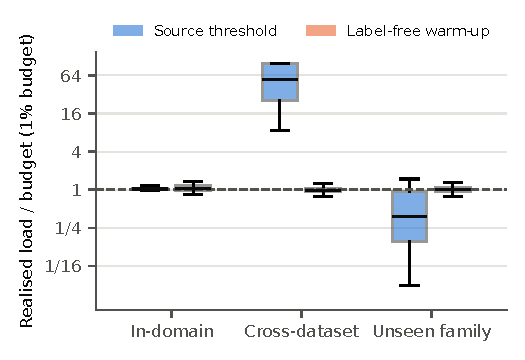
\includegraphics[width=0.55\linewidth]{../figures/budget_load.pdf}
\caption{Realised queue load relative to a 1\% review budget (log scale; 1 means the budget is met exactly). Transferred source thresholds overflow under cross-dataset shift and underfill under unseen-family shift; a quantile taken on the first 20\% of the unlabeled target stream holds the budget in every regime.}\label{fig:load}
\end{figure}

\subsection{Cost}
Scoring a flow with a detector plus the kNN novelty model takes a median of 35--40\,\textmu s per flow on four CPU cores, measured end to end in our Python pipeline, so the triage layer is cheap enough for flow-level deployment.

\section{Discussion}\label{sec:discussion}

\subsection{What the joint view shows that single-axis evaluations miss}
Evaluated one axis at a time, our models look deployable. In-domain AUROC is near 1, calibration error is near 0, and the thresholds hit their nominal false-positive rate. Viewed jointly, three problems appear that a single-axis evaluation would not reveal.
\begin{itemize}
\item \emph{Calibration does not transfer.} It is a property of the pair of source and target distributions, not of the model. Post-hoc recalibration on source data, the usual fix, leaves cross-dataset ECE at 0.28--0.45. Well-calibrated in-domain probabilities should therefore not be used to plan alert volumes on a new network, consistent with observations outside security~\cite{ovadia2019trust}.
\item \emph{Ranking metrics hide operational failure.} The same average AUROC can come with a thirtyfold alarm flood (CSE-CIC-IDS2018$\to$CIC-IDS2017) or with near-total silence (ACI-IoT-2023$\to$CIC-IDS2017). This extends Jin and Lee's observation of threshold collapse~\cite{jin2026benchmark} to a failure mode that is arguably worse, because a silent detector raises no suspicion.
\item \emph{Unseen-family misses are a thresholding problem more than a representation problem.} The held-out family usually ranks above benign traffic but below the operating threshold. Almost a third of families are missed, and almost a quarter (11 of 47) are missed with high calibrated confidence, so uncertainty-based rejection alone~\cite{talpini2024enhancing} would not flag them.
\end{itemize}

\subsection{Implications for practice}
Four recommendations follow from the results.
\begin{enumerate}
\item \emph{Fix volume, not score.} Define the alert policy as a review budget and enforce it with a quantile of the priority on recent unlabeled traffic. This costs nothing and kept the median queue size within 5\% of plan under every shift we tested, whereas thresholds carried over from training were off by factors of 0.4 to 54.
\item \emph{Treat novelty evidence as insurance.} Fusing a benign-referenced novelty p-value with the detector p-value (Fisher's method) roughly doubles recall at a 1\% budget on the families the detector misses, at a cost of 2--6 points on families it already detects. Whether that trade is worth it depends on the relative cost of a missed campaign and a slightly less efficient queue; in many SOCs a missed zero-day is the costlier error. A practical middle ground is to reserve a small fixed share of the budget for novelty-ranked flows. This is the budget-splitting analogue of the Bonferroni rule and a natural next step.
\item \emph{Do not expect any post-hoc layer to rescue cross-network transfer.} Neither calibration nor novelty fusion recovered cross-dataset recall; the models had learned features specific to how each capture was generated. Local retraining, or at least local benign reference data for the novelty score, remains necessary.
\item \emph{Report at realistic base rates.} Precision at 1\% prevalence was at most 0.49 even in-domain, and about 0.03 across datasets. Balanced-test accuracy says little about analyst workload~\cite{axelsson2000base,alahmadi2022falsepositives}.
\end{enumerate}

\subsection{Choice of novelty reference}
The novelty score should measure distance to \emph{benign} traffic, as the null hypothesis requires. In a first complete run of Protocol OS we used all training flows, including attacks, as the kNN reference. Because unseen attacks often resemble known ones, that choice made them look typical: the mean AUROC between held-out-family flows and benign flows was 0.74, against 0.83 with the benign reference (both runs are released). The difference was largest on UNSW-NB15, where the median rose from 0.52 to 0.91. We report the benign-reference variant throughout. The kNN score is also blind to some attacks. Floods and sweeps in ACI-IoT-2023 consist of very short, highly regular flows that lie \emph{closer} to benign traffic than benign flows lie to each other (novelty AUROC below 0.5 for SYN flood and ping sweep in a pilot). Detecting such hyper-typical traffic needs volumetric or host-level context that per-flow features do not carry.

\subsection{Threats to validity}\label{sec:threats}
\emph{Data availability.} Network restrictions in our execution environment prevented us from obtaining the NetFlow-v2 versions of several datasets~\cite{sarhan2022standard}, the full CIC-IDS2017 release and the full ToN-IoT normal class. We used a published subsample of CIC-IDS2017 and a ToN-IoT copy with 50{,}000 of the 300{,}000 normal records; the ACI-IoT-2023 file came from a public mirror whose class counts match the official release. All provenance, including checksums, is released. Because all operational metrics are computed on streams resampled to a fixed prevalence, these choices affect the diversity of benign training data but not the definitions of the metrics. Known labelling problems in CIC-IDS2017 and CSE-CIC-IDS2018~\cite{engelen2021troubleshooting,lanvin2023errors,flood2024bad} also affect our results; we did not relabel the data.

\emph{Feature alignment.} The three CICFlowMeter datasets were produced with different tool versions, and some features differ in implementation, not only in traffic. This is part of what a practitioner faces when moving a model between networks, but it means our cross-dataset results mix network shift with tooling shift.

\emph{Scope of models and splits.} We used four standard tabular model families, which remain strong on this kind of data~\cite{grinsztajn2022tree}, and random stratified splits within datasets. Temporal splits~\cite{pendlebury2019tesseract,luay2025temporal}, deep sequence or graph models, and adaptive conformal methods for drifting streams~\cite{gibbs2021adaptive,barber2023conformal} are natural extensions. The unseen-family protocol used LightGBM only, and the grouping in Table~\ref{tab:gain} is post hoc.

\emph{Guarantees.} The conformal false-alarm guarantee holds only under exchangeability of benign target and calibration flows. Our cross-dataset results show that this assumption fails across networks, which is why we fix the budget empirically rather than relying on the nominal $\alpha$.

\section{Conclusion}\label{sec:conclusion}

We evaluated ML-based intrusion detectors jointly under cross-dataset shift, unseen attack families and calibration, from the viewpoint of a SOC with a fixed review budget. Near-perfect in-domain scores did not carry over to the operational questions. Across networks, ranking fell to near chance, calibration error rose tenfold or more and could not be repaired on source data, and the alert threshold either flooded analysts with 5--32 times the planned false alarms or went almost silent. Within a network, 30\% of held-out attack families were detected less than half of the time, often with high calibrated confidence. Two simple measures help. A review budget enforced with a quantile of recent unlabeled traffic keeps the analyst queue at its planned size under every shift we tested. Fusing a benign-referenced novelty p-value with the detector's p-value roughly doubles recall at a 1\% budget on the attack families the detector misses, at a small cost on the families it already detects. Neither measure substitutes for local data when a model moves to a new network. We release all code, data provenance and results so that the protocol can be applied to new detectors and datasets.

\section*{CRediT authorship contribution statement}
% TODO(author): adjust to the actual contributions.
\textbf{Osman Can Çetlenbik:} Conceptualization, Methodology, Software, Validation, Formal analysis, Investigation, Data curation, Visualization, Writing -- original draft.
\textbf{Ahmet Ali Süzen:} Conceptualization, Supervision, Validation, Writing -- review \& editing.

\section*{Declaration of competing interest}
The authors declare that they have no known competing financial interests or personal relationships that could have appeared to influence the work reported in this paper.

\section*{Data and code availability}
All datasets used are publicly available from their original providers. The code, the exact data provenance (source URLs, commit hashes and MD5 checksums), the processed-data summaries and all raw result tables are available at \url{https://github.com/osmancancet/nids-budgeted-triage}.

\section*{Declaration of generative AI and AI-assisted technologies in the writing process}
% Required by Elsevier. TODO(author): review and adapt this statement to reflect your actual use.
During the preparation of this work the author(s) used Claude (Anthropic), an AI assistant, to help with literature search, code development, running experiments, and drafting and editing the manuscript. After using this tool, the author(s) reviewed and edited the content as needed and take(s) full responsibility for the content of the published article.

\section*{Acknowledgements}
% TODO(author): funding and acknowledgements.


\bibliographystyle{elsarticle-num}
\bibliography{refs}

\end{document}
